\documentclass [12pt]{article}
\setlength{\parindent}{0em}
\setlength{\parskip}{0.25in}
\usepackage{geometry}
\geometry{verbose,letterpaper,tmargin=0.5in,bmargin=1.0in,lmargin=.70in,rmargin=.70in}
\usepackage{graphicx}
\usepackage{amsmath}
\usepackage{amssymb}
\usepackage{amsthm}
\theoremstyle{definition}
\newtheorem{exmp}{Example}[section]
\usepackage{tikz}
\usetikzlibrary{arrows,decorations.pathmorphing,backgrounds,positioning,fit,petri,calc,matrix}
\usepackage{slashbox}
\usepackage{listings}
\usepackage{ dsfont }
\usepackage{ upgreek }
\usepackage{graphicx}
\graphicspath{ {./images/} }


\newcommand{\ket}[1]{| {#1} \rangle}
\newcommand{\bra}[1]{\langle {#1} |}
\newcommand{\braket}[2]{\langle #1 \ | \ #2 \rangle}
\newcommand{\qp}[2]{\langle #1 \ | \ #2 \ | \ #1 \rangle}
\newcommand{\tensor}[2]{ #1 \otimes  #2 }
\newcommand{\iz}[1]{\mathds{#1}^{n}}
\newcommand{\md}[1]{|#1|}
\newcommand{\suml}[2]{\sum\limits_{#1}^{#2}}

\definecolor{dkgreen}{rgb}{0,0.6,0}
\definecolor{gray}{rgb}{0.5,0.5,0.5}
\definecolor{mauve}{rgb}{0.58,0,0.82}

\lstset{frame=tb,
  language=Python,
  aboveskip=3mm,
  belowskip=3mm,
  showstringspaces=false,
  columns=flexible,
  basicstyle={\small\ttfamily},
  numbers=none,
  numberstyle=\tiny\color{gray},
  keywordstyle=\color{blue},
  commentstyle=\color{dkgreen},
  stringstyle=\color{mauve},
  breaklines=true,
  breakatwhitespace=true,
  tabsize=3
}

\DeclareMathOperator{\Cspan}{ \CC-span }

\title{Home Work 11}
\author{Madhu Peduri}
\date{04/27/2021}

\begin{document}
\section*{Homework 11}

{\bf 1.1.} Prove that $x^{t} -1 = (x-1)\suml{k=0}{t-1} x^{k}$

\phantom{1em} {\bf 1.} Consider the polynomial $1 + x + \dots + x^{t-1}$

\phantom{1000em} $\Rightarrow (1 + x + \dots + x^{t-1}) \dfrac{(x-1)}{(x-1)}$

\phantom{1000em} $\Rightarrow \dfrac{(x + x^{2} + \dots + x^{t-1} + x^{t} - 1 - x - x^{2} - \dots - x^{t-1})}{(x-1)}$

\phantom{1000em} $\Rightarrow 1 + x + \dots + x^{t-1} = \dfrac{(x^{t} -1)}{(x-1)}$

\phantom{1000em} $\Rightarrow \suml{k=0}{t-1} x^{k} = \dfrac{(x^{t} -1)}{(x-1)}$

\phantom{1em} {\bf 2.} $x^{t} -1 = (x-1)\suml{k=0}{t-1} x^{k}$

{\bf 1.2.} Prove that $x=e^{2\Uppi i(m/t)}$ is the solution to $x^{t} - 1$ for $m \in \mathds{Z}$

\phantom{1em} {\bf 1.} Substitute $e^{2\Uppi i(m/t)}$ in the equation $x^{t} - 1$

\phantom{1000em} $\Rightarrow x^{t} - 1 = (e^{2\Uppi i(m/t)})^{t} - 1 = e^{2\Uppi i \frac{mt}{t}} - 1 = (e^{i2 \Uppi})^{m} - 1$

\phantom{1em} {\bf 2.} We know that,\\
\phantom{1000em} $e^{i\theta} = cos(\theta) + isin(\theta)$ and \\
\phantom{1000em} $(cos(\theta) + isin(\theta))^{m} = cos(m\theta) + isin(m\theta)$

\phantom{1000em} $\Rightarrow x^{t} - 1 = (e^{i2 \Uppi})^{m} - 1 = cos(2 \Uppi m) + isin(2 \Uppi m) - 1$

\phantom{1em} {\bf 3.} if $m \in \mathds{Z}$, then \\
\phantom{1000em} $cos(2 \Uppi m) = 1$ and $sin(2 \Uppi m) = 0$

\phantom{1000em} $\Rightarrow x^{t} - 1 = cos(2 \Uppi m) + isin(2 \Uppi m) - 1 = 1 + 0 - 1 = 0$

\phantom{1em} {\bf 4.} Thus $e^{2\Uppi i(m/t)}$ is the root for the equation $x^{t} - 1$ for $m \in \mathds{Z}$

\newpage

{\bf 1.3.} Prove that $\suml{k=0}{t-1} e^{2\Uppi i(km/t)} = 
	\begin{cases}
   		t & \text{if } m = 0, \\
     	0 & \text{otherwise}.
    \end{cases}$

\phantom{1em} {\bf 1.} When $m = 0$, $e^{2\Uppi i(m/t)} = 1$\\
\phantom{1000em} $\suml{k=0}{t-1} e^{2\Uppi i(km/t)} = 1 + 1 + \dots + t-1$, \\
\phantom{1000em} $\Rightarrow \suml{k=0}{t-1} e^{2\Uppi i(km/t)} = t$

\phantom{1em} {\bf 2.} When $m \neq 0$ and $0 \leq m \leq t$,\\
\phantom{1000em} $\suml{k=0}{t-1} e^{2\Uppi i(km/t)} = \suml{k=0}{t-1} (e^{2\Uppi i(m/t)})^{k}$\\
\phantom{1000em} $\Rightarrow \suml{k=0}{t-1} (e^{2\Uppi i(m/t)})^{k} = \dfrac{(e^{2\Uppi i(m/t)})^{t} - 1}{e^{2\Uppi i(m/t)} - 1}$, using 1.1

\phantom{1em} {\bf 3.} From 1.2, we know that, $e^{i 2\Uppi m} = 1$

\phantom{1000em} Thus for $m \neq 0$ and $0 \leq m \leq t$,\\
\phantom{1000em} $\Rightarrow \suml{k=0}{t-1} (e^{2\Uppi i(m/t)})^{k} = \dfrac{e^{i2\Uppi m} - 1}{e^{2\Uppi i(m/t)} - 1} = \dfrac{1 - 1}{e^{2\Uppi i(m/t)} - 1} = 0$

{\bf 2.} By given definition, $QFT\ket{x} = \dfrac{1}{\sqrt{2^{n}}} \bigotimes_{k=1}^{n}(\ket{0} + e^{\frac{i2\Uppi [x]}{2^{k}}}\ket{1})$ 

\phantom{1em} {\bf 1.} We rearrage the definition of QFT using summation and product as below,

\phantom{1000em} $QFT = \dfrac{1}{\sqrt{2^{n}}} \suml{j=0}{2^{n} - 1}[ \prod\limits_{k=1}^{n} e^{\frac{i2\Uppi [x]}{2^{k}}}] \ket{j_{1} j_{2} \dots j_{n}}$

\phantom{1000em} In above equation, we can rewrite the product component as below \\
\phantom{1000em} $\prod\limits_{k=1}^{n} e^{\frac{i2\Uppi [x]}{2^{k}}} = e^{i2\Uppi \alpha}$ where $\alpha = \suml{l=1}{n} \dfrac{j_{l}}{2^{l}}$

\phantom{1em} {\bf 2.1.} If we perform QFT on $\ket{0^{n}}$ , then 

\phantom{1000em} $\alpha = 0$, because, $j_{l} = 0$

\phantom{1000em} $\Rightarrow \prod\limits_{k=1}^{n} e^{\frac{i2\Uppi [x]}{2^{k}}} = e^{i2\Uppi \alpha} = 1$

\phantom{1000em} $\Rightarrow QFT\ket{0^{n}} =  \dfrac{1}{\sqrt{2^{n}}} \suml{j=0}{2^{n} - 1} \ket{j_{1} j_{2} \dots j_{n}} = \dfrac{1}{\sqrt{2^{n}}} \suml{j \in \{0,1\}^{n}}{ } \ket{j}$

\phantom{1em} {\bf 2.2.} If we perform QFT on $\ket{1^{n}}$ , then

\phantom{1000em} $\alpha = \suml{l=1}{n} \dfrac{j_{l}}{2^{l}} = \dfrac{[1 + 2 + 2^{2} + \dots + 2^{k-1}]}{2^{k}} = \dfrac{[j]}{2^{k}}$

\phantom{1000em} $\Rightarrow QFT\ket{1^{n}} = \dfrac{1}{\sqrt{2^{n}}} \suml{j=0}{2^{n} - 1} e^{\dfrac{i2\Uppi [j]}{2^{k}}} \ket{j_{1} j_{2} \dots j_{n}} = \dfrac{1}{\sqrt{2^{n}}} \suml{j \in \{0,1\}^{n}}{ } e^{\dfrac{i2\Uppi [j]}{2^{k}}} \ket{j}$

{\bf 3.} We have $QFT\ket{x} = \dfrac{1}{\sqrt{2^{n}}} \bigotimes_{k=1}^{n}(\ket{0} + e^{\frac{i2\Uppi [x]}{2^{k}}}\ket{1})$

\phantom{1em} {\bf 1.} We rearrage the definition of QFT using summation and product as below,

\phantom{1000em} $QFT\ket{x} = \dfrac{1}{\sqrt{2^{n}}} \suml{y=0}{2^{n} - 1}[ \prod\limits_{k=1}^{n} e^{\frac{i2\Uppi [x]}{2^{k}}}] \ket{y_{1} y_{2} \dots y_{n}}$

\phantom{1000em} In above equation, we can rewrite the product component as below \\
\phantom{1000em} $\prod\limits_{k=1}^{n} e^{\frac{i2\Uppi [x]}{2^{k}}} = e^{i2\Uppi [x] \alpha}$ where $\alpha = \suml{l=1}{n} \dfrac{y_{l}}{2^{l}}$

\phantom{1em} {\bf 2.} If we consider, $\alpha = \suml{l=1}{n} \dfrac{y_{l}}{2^{l}} = [y]$ where $[x],[y]$ are binary decimal representations. 

\phantom{1000em} $\Rightarrow QFT\ket{x} = \dfrac{1}{\sqrt{2^{n}}} \suml{j=0}{2^{n} - 1} e^{\frac{i2\Uppi [x][y]}{2^{k}}} \ket{y_{1} y_{2} \dots y_{n}}$
 
\phantom{1000em} $\Rightarrow QFT\ket{x} = 2^{-n/2} \suml{y \in \{0,1\}^{n}}{ } e^{\dfrac{i2\Uppi [x][y]}{2^{n}}} \ket{y}$
 
\newpage
 
{\bf 4.} \\
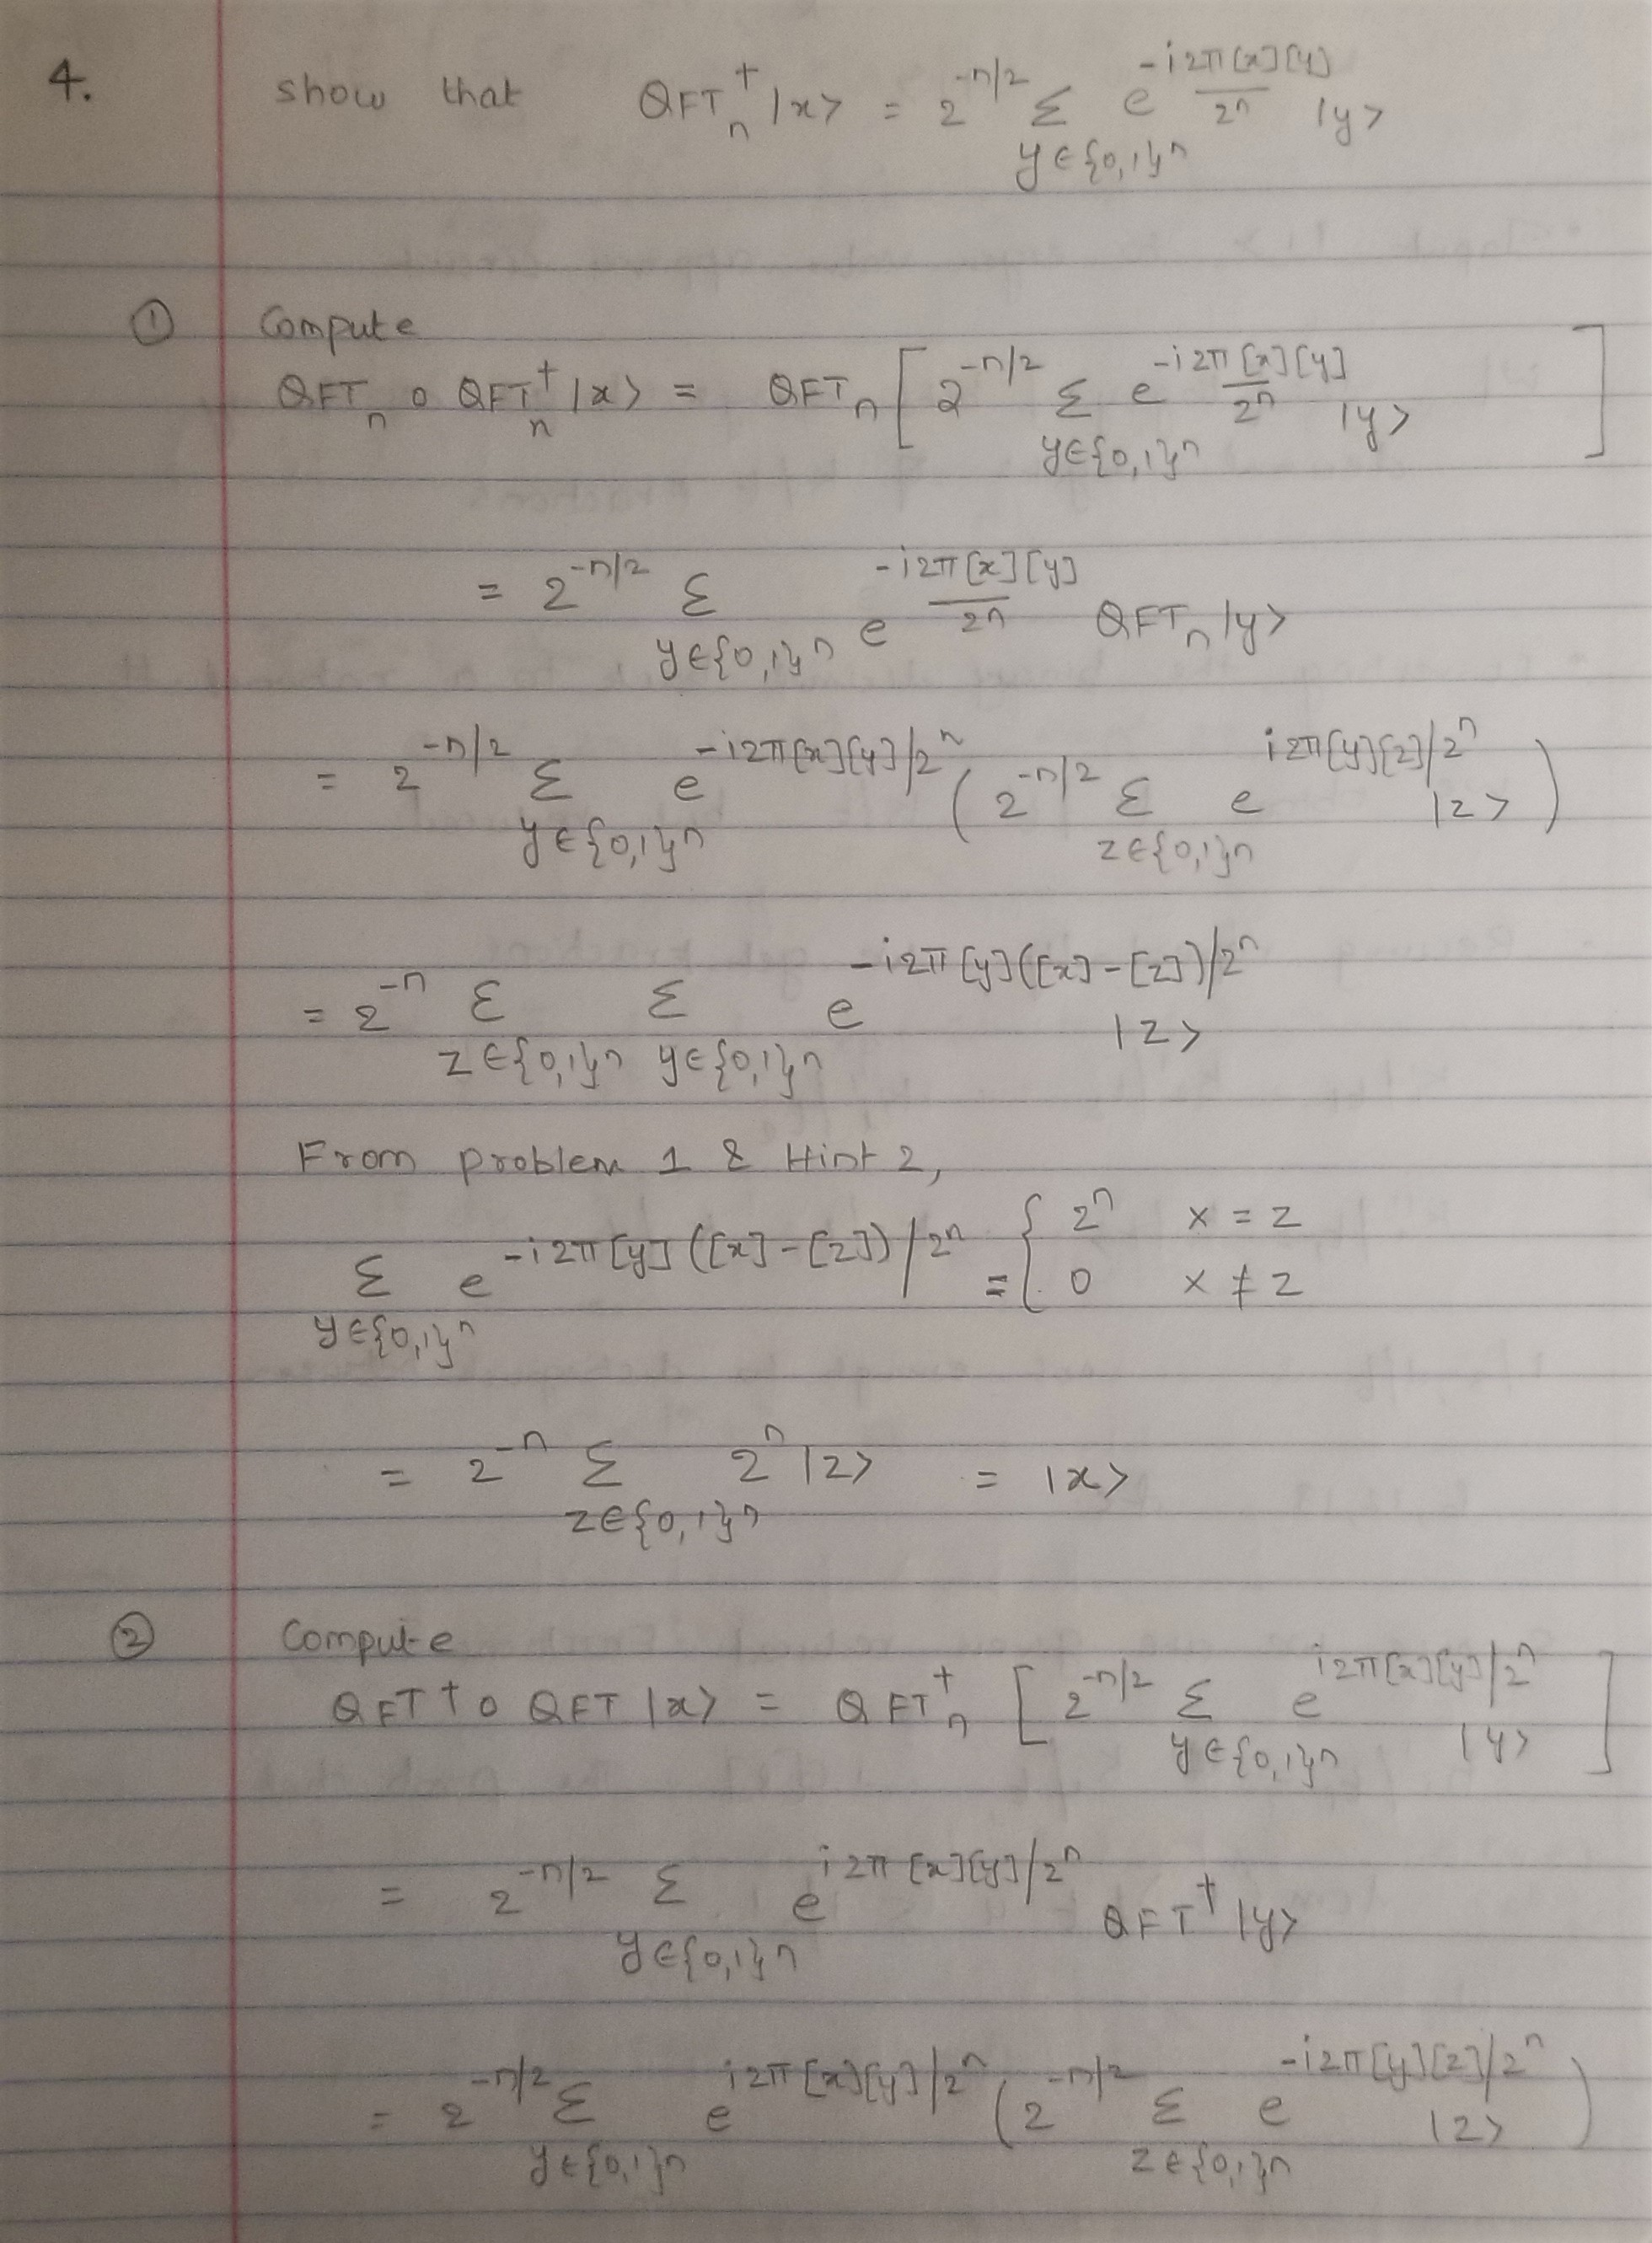
\includegraphics[width=18cm, height=23cm]{I1}
\newpage
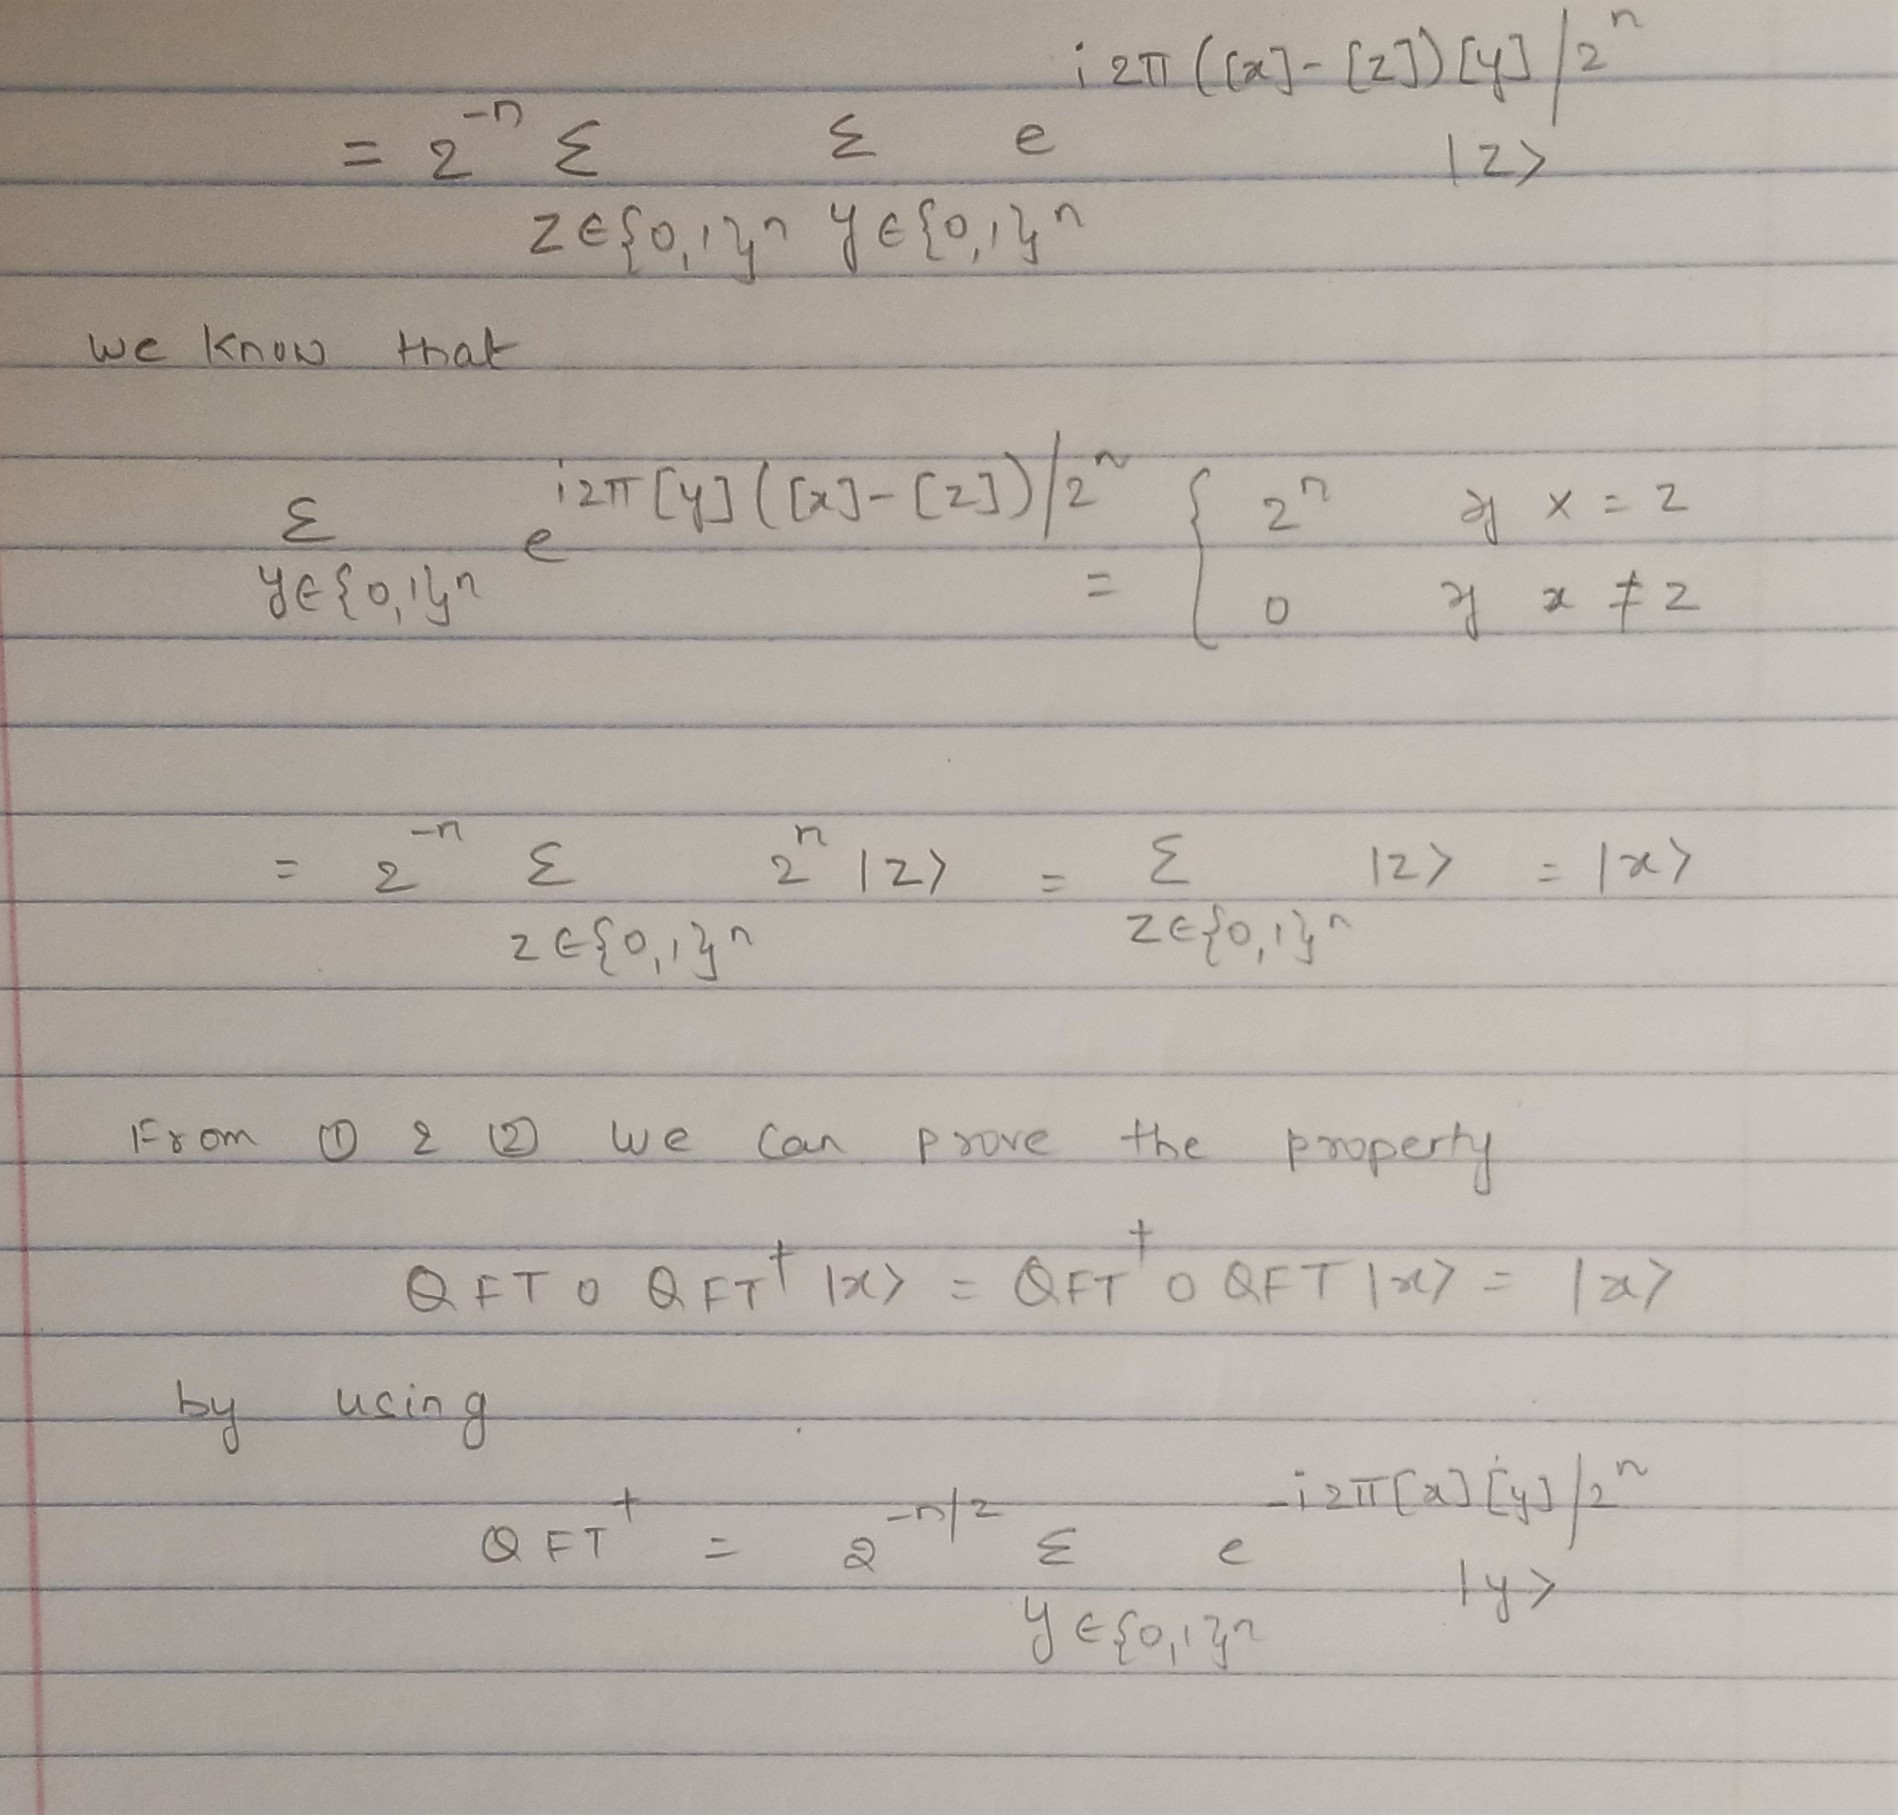
\includegraphics[width=18cm, height=23cm]{I2}

\newpage

{\bf 5.} \\
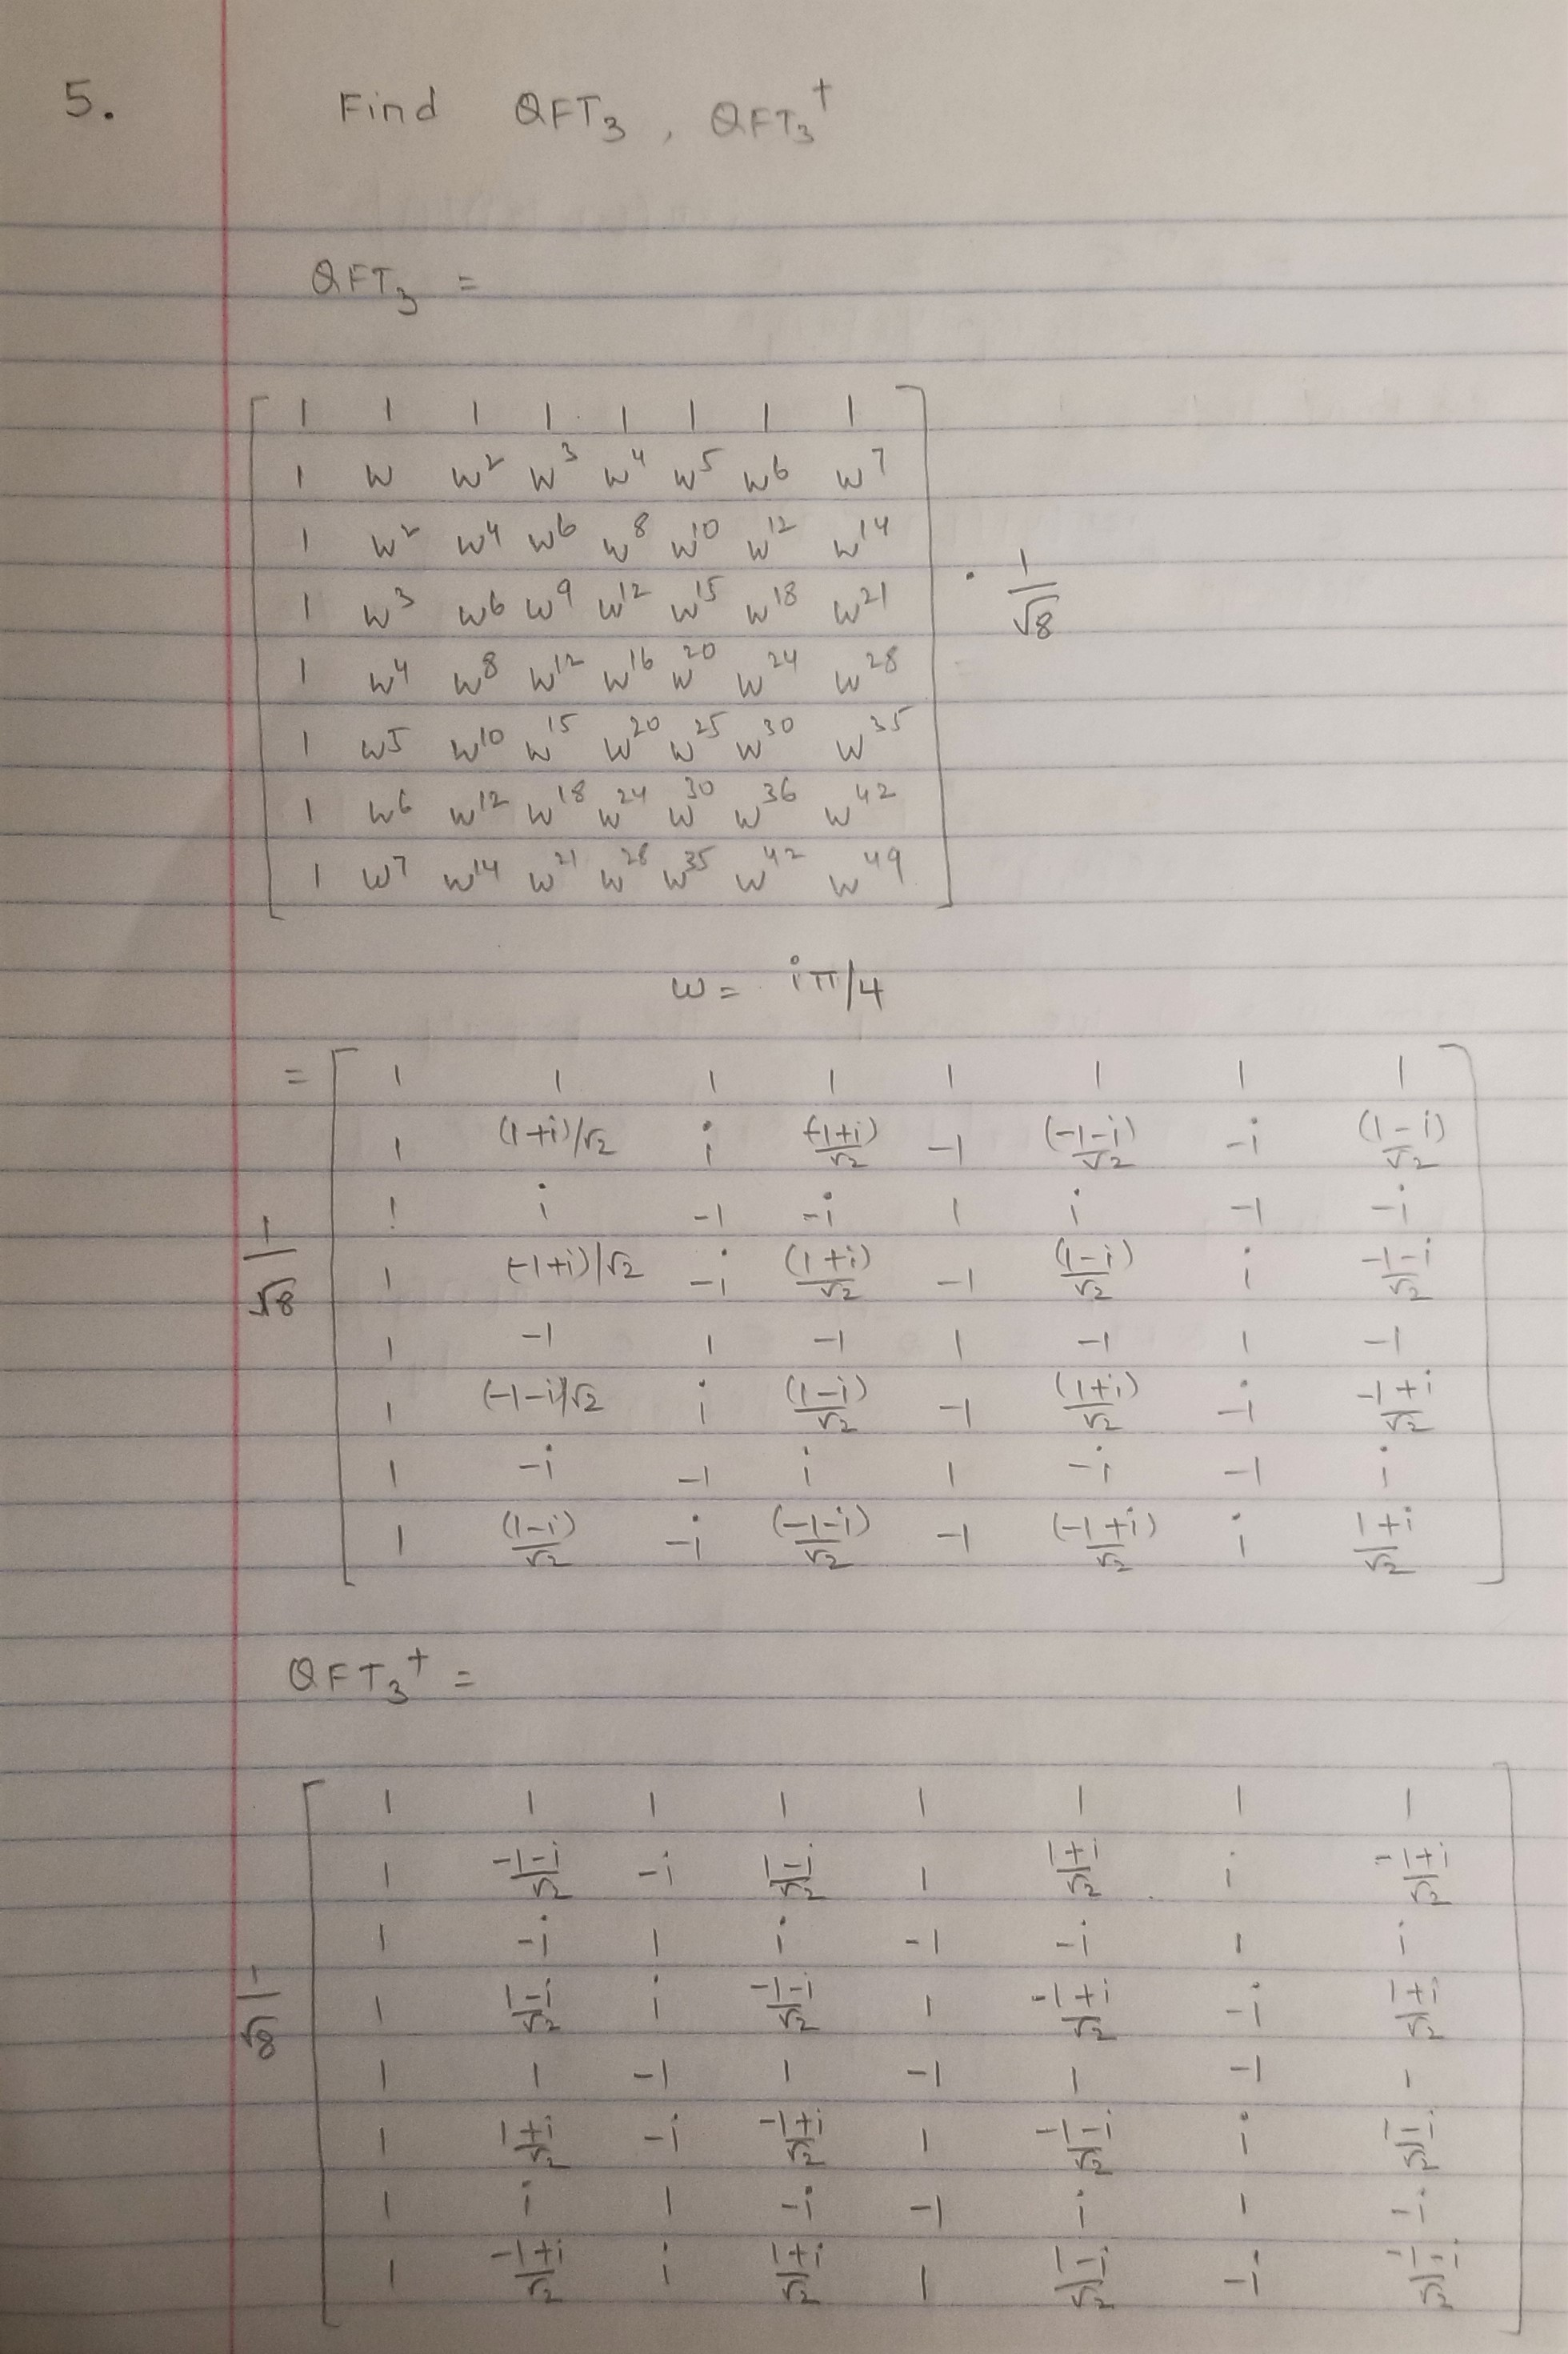
\includegraphics[width=18cm, height=23cm]{I3}

\end{document}